%        File: ans_2013_therm.tex
%     Created: Mon Aug 13 10:00 AM 2012 C
%

%% To use the glossaries acronym package, you'll need to define any acronyms you intend to 
%% use. You can define acronyms with \newacronym{label}[acronym]{written out form}
%% To refer to them in the text use \gls{label}

\documentclass{anstrans}
%%%%%%%%%%%%%%%%%%%%%%%%%%%%%%%%%%%
\usepackage[acronym,toc]{glossaries}
\makeglossaries

% concise yet adequately descriptive title
\title{Rapid Determination of Thermal Repository Capacity For Fuel Cycle Analysis}
\author{Kathryn D.~Huff$^1$, Alexander T. Bara$^2$}

%% uncomment these next five only if using anstrans
\institute{$^1$Univ. of Wisconsin, 1500 Engineering Dr., Madison, WI, 53706\\ 
\& Argonne National Laboratory, 9700 S. Cass Ave., Lemont, IL, katyhuff@gmail.com\\
$^2$Univ. of Illinois, Urbana Champaign, IL, 61801, bara1@illinois.edu}
\usepackage{graphicx}
\usepackage{booktabs} % nice rules for tables
\usepackage{microtype} % if using PDF
\newcommand{\units}[1] {\:\text{#1}}%
\newcommand{\SN}{S$_N$}%{S$_\text{N}$}%{$S_N$}%

\date{}
%%%%%%%%%%%%%%%%%%%%%%%%%%%%%%%%%%%
\begin{document}
%%%%%%%%%%%%%%%%%%%%%%%%%%%%%%%%%%%%%%%%%%%%%%%%%%%%%%%%%%%%%%%%%%%%%%%%%%%%%%%%
\section{Introduction}
% Provide a summary of the work conducted:
%      Describe the technical problem clearly
%      support it with a method

An algorithm for rapid thermal repository capacity calcuation implemented in Cyder, a 
software library for coupled thermal and hydrologic repository performance 
analysis is described. Integration of Cyder with the Cyclus fuel cycle simulator 
is also described. Finally, a proof of principle demonstration is presented in 
which the rapid calculation method described here is benchmarked against results 
of a more detailed model.

This algorithm employs a specific temperature change method \cite{radel} and has 
resulted from combining detailed spent nuclear fuel composition data with 
detailed thermal repository performance analysis tools from the \gls{UFD} 
campaign, \gls{LLNL}, and \gls{ANL}\cite{radel,llnl,sinda,carter}. By 
abstraction of these detailed thermal models, Cyder captures the dominant 
physics of thermal phenomena affecting repository capacity in various geologic 
media and as a function of spent fuel composition.

Abstraction of detailed computational thermal repository performance model 
calculations has resulted in a reference dataset and an associated specific 
temperature change estimation. This method is capable of rapid estimation of 
temperature increase near emplacement tunnels as a function of waste 
composition, waste package spacing, near field thermal conductivity, and near 
field thermal diffusitivity. 

\section{Motivation}
% Provide a brief description of the importance of the work (what problem it 
%   addresses/solves):

Thermal evolution of a geologic repository is a strong function of spent fuel 
composition, which varies among alternative fuel cycles. For this reason, a 
generic disposal model capable of dynamic integration with a systems analysis 
framework is necessary to illuminate capacity constraints and dynamic feedback 
effects of candidate repository geologies in the context of fuel cycle options.
In answer to this need, the algorithm in this work has been implemented in the 
open source Cyder software library which integrates with the Cyclus computational 
fuel cycle systems analysis platform \cite{huff_cyder_2012,huff_cyclus:_2010}. 

A generic repository model appropriate for systems analysis must emphasize 
modularity and speed while providing modeling options at various levels of 
detail. Parameterized simulations and abstraction efforts conducted to develop 
the method described in this work sought to capture the dominant physics of 
thermal repository capacity assessment so that the Cyder disposal environment 
library could meet the simulation speed required by the Cyclus fuel cycle 
simulator.

\section{Methodology}
  % table?
  Important heat limits in materials of the repository restrict loading designs 
  and capacity.
  %        File: heat_tab.tex
%     Created: Thu Aug 04 11:00 AM 2011 C
% Last Change: Thu Aug 04 11:00 AM 2011 C
%
\begin{table}[h!]
  \centering
  \footnotesize{
  \begin{tabular}{|l|r|r|r|r|}
    \multicolumn{5}{c}{\textbf{Thermal Behavior of Various Concepts}}\\
    \hline
            & Clay & Granite & Salt & Deep \\ 
            & & & & Borehole \\ 
            & (Bentonite & (Concrete & (Salt & (Bentonite\\ 
            & Buffer) & Buffer) & Backfill) & Buffer) \\ 
    \hline
    Buffer Limit $[^{\circ}C]$ & \textbf{100}  & \textbf{100}  & \textbf{180} & \textbf{100}  \\ 
    Reference
    & \cite{hardin_generic_2011}   
    & \cite{von_lensa_red-impact_2008}   
    & \cite{von_lensa_red-impact_2008,brewitz_long-term_2002}   
    & \cite{von_lensa_red-impact_2008}  \\ 
    &      &      &     &      \\
    Host Limit $[^{\circ}C]$   & \textbf{100}  & \textbf{200}  & \textbf{180} & \textbf{none} \\ 
    Reference                     
    & \cite{andra_argile:_2005}   
    & \cite{von_lensa_red-impact_2008}   
    & \cite{hardin_generic_2011}   
    & \cite{hardin_generic_2011, brady_deep_2009}   \\
    &      &      &     &      \\
    $\alpha_{th} [\frac{10^{-6}m^2}{s}]$ & \textbf{0.12-0.19} & \textbf{0.9-1.8} & \textbf{1.3-2.1} &\textbf{ 0.9-1.8} \\ 
    Reference                     
    & \cite{tikhonravova_effect_2007} 
    & \cite{durham_thermal_1987,hardin_generic_2011,kim_thermal_2007}     
    & \cite{hardin_generic_2011,nieland_storage_2001}   
    & \cite{durham_thermal_1987,hardin_generic_2011,kim_thermal_2007}   \\ 
    &      &      &     &      \\
    $K_{th} [\frac{W}{m{\cdot}K}]$ & \textbf{1-2} & \textbf{2-4} & $\mathbf{\sim4}$  & \textbf{2-4} \\ 
    Reference                     
    & \cite{hardin_generic_2011,tikhonravova_effect_2007}    
    & \cite{hardin_generic_2011,kim_thermal_2007,surma_porosity_2003,ab_long-term_2006}    
    & \cite{hardin_generic_2011,nieland_storage_2001}
    & \cite{hardin_generic_2011,kim_thermal_2007,surma_porosity_2003}\\ 
    &      &      &     &      \\
    Coalescence & yes & no & yes & no \\ 
    \hline
  \end{tabular}
  \caption[Models for Heat Transport for Various Geologies]{Maximum heat load constraints, thermal 
  diffusivity, and thermal conductivities vary among repository concepts and host formations. }
  \label{tab:heat_tab}
  }
\end{table}


  Similar heat transport models can be used for all geologies, but are 
  differentiated by material parameters $(c_p, K, \rho)$ and varying 
  thermal limits.

To inform dynamic behavior within the simulator, the repository requires 
a transient model capable of quickly arriving at a heat based 
capacity for an arbitrary waste stream. 
\begin{figure}[htp]
  \begin{center}
    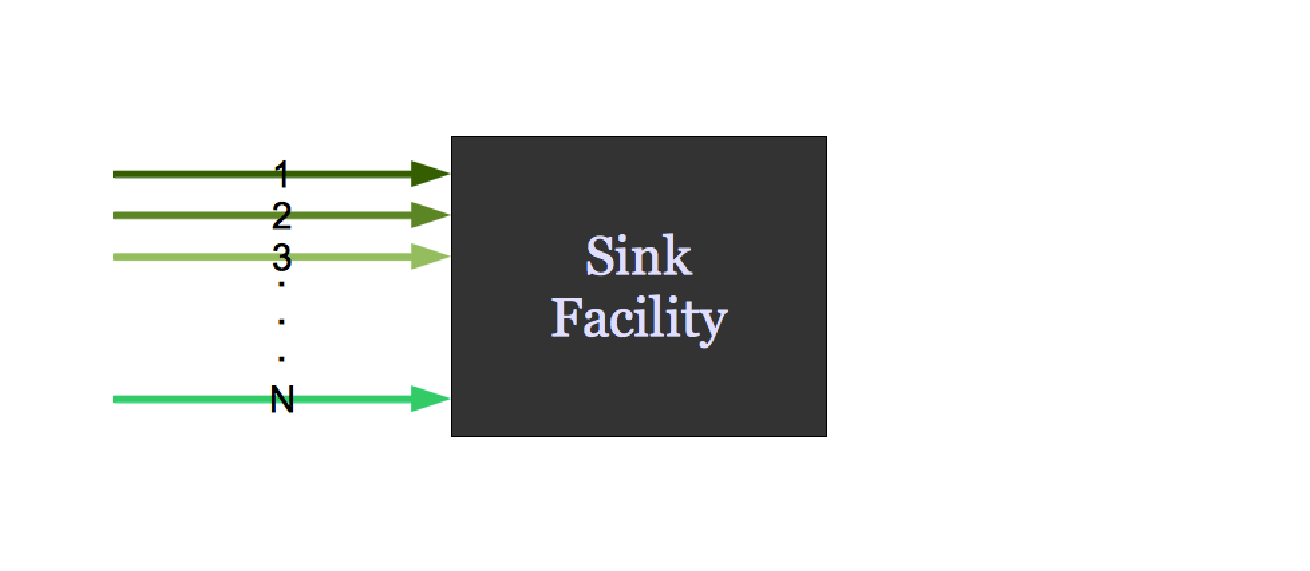
\includegraphics[width=0.7\columnwidth]{cyclus/images/sinkfacility.eps}
  \end{center}
  \caption{\footnotesize{The Cyder repository model has the same interface with the simulation 
  as does a sink facility. It receives materials according to some capacity. The 
  heat-limited capacity of the repository will be reassessed for new waste 
  streams offered to the repository.}}
  \label{fig:cydersink}
\end{figure}

\subsubsection{Specific Temperature Change Method}
Introduced by Radel, Wilson et. al., the Specific Temperature Change method uses 
a linear approximation to arrive at the thermal loading density limit.  
When the thermal time constant of the rock is much shorter than the waste form 
decay package, the change in package wall temperature can be described by 

\begin{align}
q(t_0)\rho_{limit}C'&=\Delta T_1
\intertext{where}
\rho_{limit} &= \frac{C_1}{Q_1}\nonumber\\
C' &= \mbox{ Thermal constant }[-]\nonumber\\
\Delta T &= \mbox{ Constant difference between }T_{lim}\mbox{ and }T_{amb}[^{\circ}C]\nonumber\\
T_{lim} &= \mbox{ Temperature limit }[^{\circ}C]\nonumber\\
T_{amb} &= \mbox{ Ambient rock temperature }[^{\circ}C]\nonumber
\end{align}


\begin{figure}[htp!]
\begin{center}
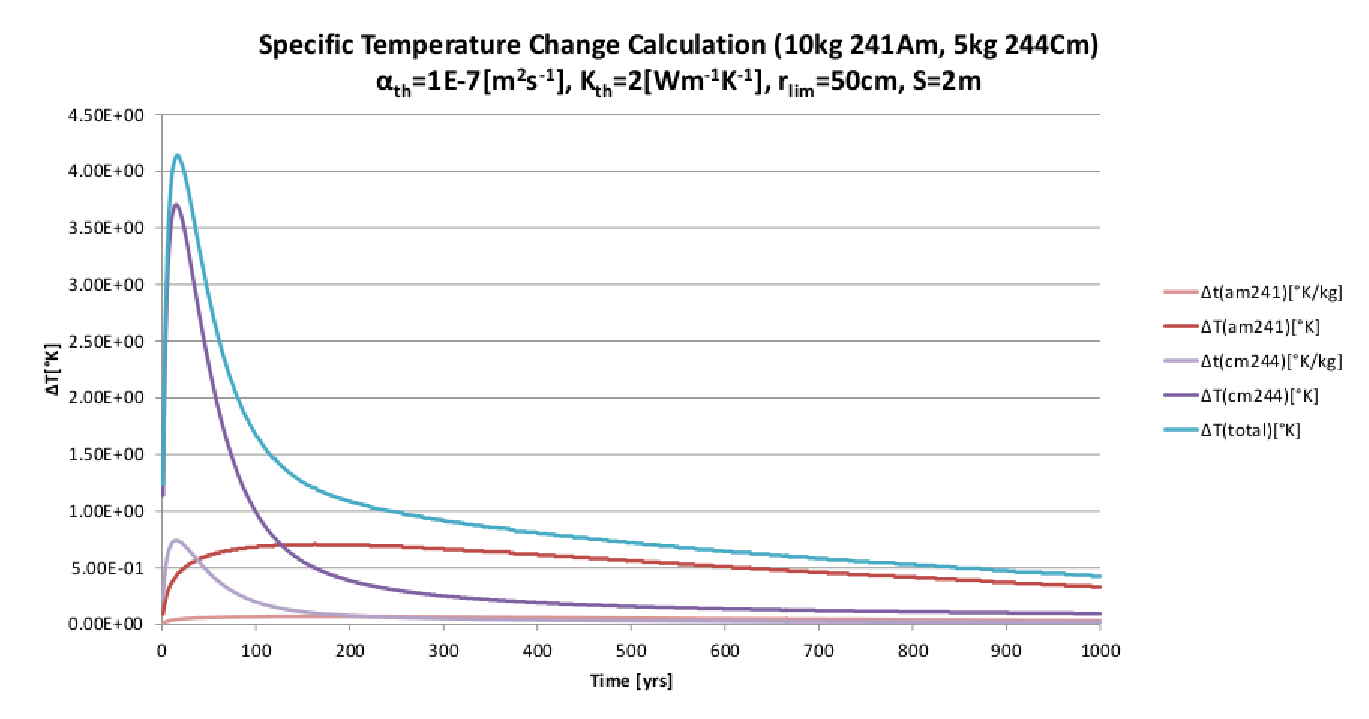
\includegraphics[width=0.8\columnwidth]{cyder/images/fakeArbitraryWF.eps}
\end{center}
\caption{\footnotesize{As a demonstration of the calculation procedure, the specific 
temperature change curves, $\Delta t$, are calculated for heat contributing 
isotopes at a 
specified repository spacing, $s$, heat limit radius, $r_{lim}$, and thermal paramters 
$\alpha_{th}$ and $K_{th}$. The total temperature change is the sum of the 
mass scaled curves $\Delta T$.}}
\label{fig:fakeArbitraryWF}
\end{figure}

Repeated runs of a detailed analytic model have given a dataset that 
facilitates estimation of thermal loading capacity for a range of thermal 
diffusitivities, conductivities, and repository layouts.
\begin{table}[ht!]
\centering
\footnotesize{
\begin{tabular}{|l|l|l|r|}
\multicolumn{4}{c}{\textbf{Thermal Cases}}\\
\hline
\textbf{Parameter} & \textbf{Symbol} & \textbf{Units} & \textbf{Value Range} \\
\hline
Diffusivity & $\alpha_{th}$ & $[m^2\cdot s^{-1}]$ & $1.0\times10^{-7}-3.0\times10^{-6}$\\
\hline
Conductivity & $K_{th}$     & $[W\cdot m^{-1} \cdot K^{-1}]$ & $0.1 - 4.5$ \\
\hline
Spacing & $S$ & $[m]$ & 2, 5, 10, 15, 20, 25, 50 \\
\hline
Radius & $r_{lim}$ & $[m]$ & 0.1, 0.25, 0.5, 1, 2, 5 \\
\hline
Isotope & $i$ & $[-]$ & $^{241,243}Am,$  \\
        & & & $^{242,243,244,245,246}Cm,$  \\
        & & & $^{238,240,241,242}Pu$  \\
        & & & $^{134,135,137}Cs$  \\
        & & & $^{90}Sr$  \\
\hline
\end{tabular}
\caption{A thermal reference dataset of \gls{STC} values as a function of each of these parameters was generated by repeated parameterized runs of the LLNL 
MathCAD model\cite{greenberg_application_2012, greenberg_investigations_2012}.}
\label{tab:thermal_cases}
}
\end{table}



\subsubsection{Supporting Thermal Response Dataset}
To support this calculation in Cyder, a reference data set of temperature change 
curves was calculated. Repeated runs of a detailed analytic model over the range of values in Table 
\ref{tab:thermal_cases} determined \gls{STC} values over a range of thermal 
heat limit radii, $r_{lim}$, thermal diffusivity values, $\alpha_{th}$,
thermal conductivity values, $K_{th}$ and waste package spacings, $S$. Linear 
interpolation across the discrete parameter space provides a simple thermal 
reference dataset for use in Cyder.

\begin{table}[ht!]
\centering
\footnotesize{
\begin{tabular}{|l|l|l|r|}
\multicolumn{4}{c}{\textbf{Thermal Cases}}\\
\hline
\textbf{Parameter} & \textbf{Symbol} & \textbf{Units} & \textbf{Value Range} \\
\hline
Diffusivity & $\alpha_{th}$ & $[m^2\cdot s^{-1}]$ & $1.0\times10^{-7}-3.0\times10^{-6}$\\
\hline
Conductivity & $K_{th}$     & $[W\cdot m^{-1} \cdot K^{-1}]$ & $0.1 - 4.5$ \\
\hline
Spacing & $S$ & $[m]$ & 2, 5, 10, 15, 20, 25, 50 \\
\hline
Radius & $r_{lim}$ & $[m]$ & 0.1, 0.25, 0.5, 1, 2, 5 \\
\hline
Isotope & $i$ & $[-]$ & $^{241,243}Am,$  \\
        & & & $^{242,243,244,245,246}Cm,$  \\
        & & & $^{238,240,241,242}Pu$  \\
        & & & $^{134,135,137}Cs$  \\
        & & & $^{90}Sr$  \\
\hline
\end{tabular}
\caption{A thermal reference dataset of \gls{STC} values as a function of each of these parameters was generated by repeated parameterized runs of the LLNL 
MathCAD model\cite{greenberg_application_2012, greenberg_investigations_2012}.}
\label{tab:thermal_cases}
}
\end{table}



The analytic model used to populate the reference dataset was created at 
\gls{LLNL} for the \gls{UFD} campaign. In this tool, heat limited thermal 
response is calculated analytically for each geology, for many waste package 
loading densities, and for many fuel cycle options \cite{hardin_generic_2011, 
greenberg_investigations_2012, greenberg_application_2012}. It employs an 
analytic model from Carslaw and Jaeger and is implemented in MathCAD 
\cite{carslaw_conduction_1959, ptc_mathcad_2010}.  The integral solver in the 
MathCAD toolset is the primary calculation engine for the analytic MathCAD 
thermal model, which relies on superposition of point, finite-line, and line 
source integral solutions.  

%The transient state of the temperature at the calculation radius is found with a convolution of the transient far field solution with the steady state near field solution.  The process is then iterated with a one year resolution in order to arrive at a temperature evolution over the lifetime of the repository. 
%
%In a two dimensional grid of waste packages, the central package is represented by the finite line solution

Figure \ref{fig:CmScaling} demonstrates the scaling of an STC curve according to 
equation \eqref{STC} to represent the heat from $25.9g$ of initial $^{242}Cm$ using 
the reference data set. 

\begin{figure}[h!]
\begin{center}
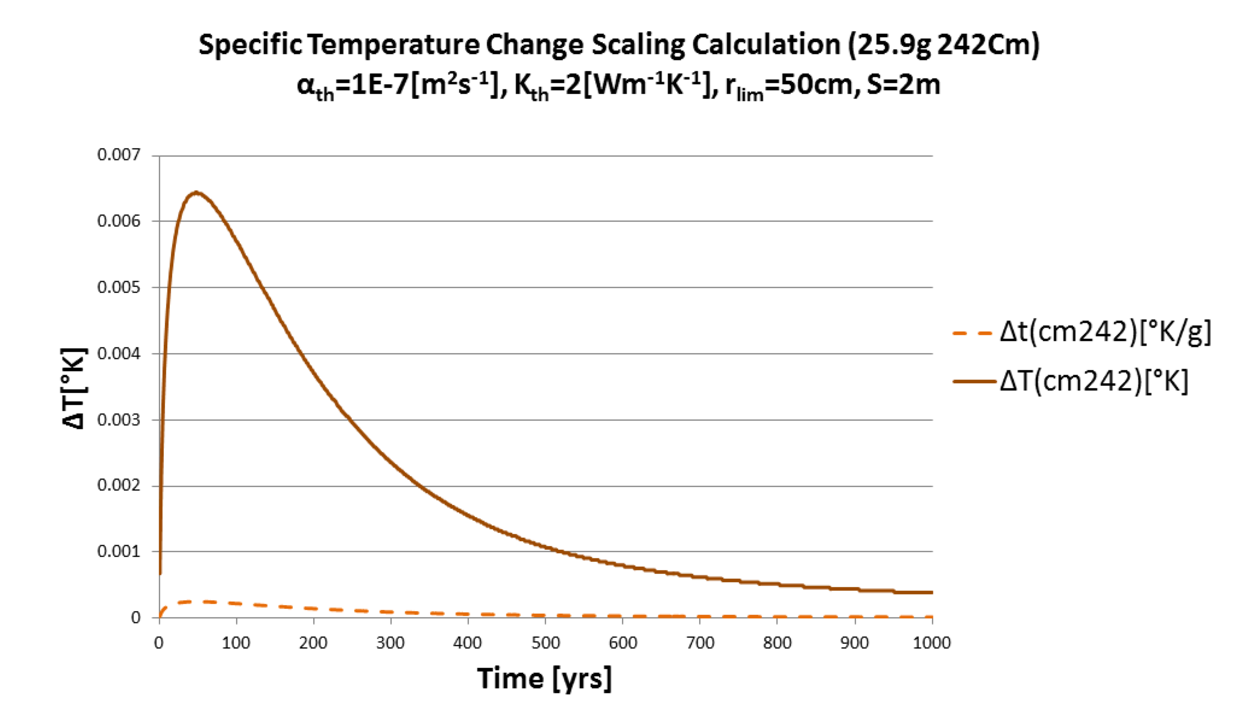
\includegraphics[width=\columnwidth]{images/CmScaling.eps}
\end{center}
\caption{As a demonstration of the calculation procedure, the temperature change 
  curve for one initial gram of $^{242}Cm$ and is scaled to represent $25.9g$, 
  approximately the $^{242}Cm$ inventory per MTHM in 51GWd burnup UOX PWR fuel. }
\label{fig:CmScaling}
\end{figure}


The supporting database was limited to  high heat contributing isotopes, $H$, 
such that the superposition in equation \eqref{superposition} becomes 

\begin{align}
\Delta T (r_{lim},S,K_{th},\alpha_{th})&\sim \sum_{i\in H} m_i \Delta t_i(r_{lim},S,K_{th},\alpha_{th})
\label{superposition_approx}
\intertext{where}
H &= \mbox{ set of high heat isotopes }[-]\nonumber\\
S &= \mbox{ uniform waste package spacing } [m]\nonumber\\
K_{th} &= \mbox{ thermal conductivity } [W\cdot m^{-1}\cdot K^{-1}]\nonumber\\
\alpha_{th} &= \mbox{ thermal diffusivity } [m^2\cdot s^{-1}]\nonumber\\
\end{align}

The use of this superposition is demonstrated in Figure 
\ref{fig:CmSuperposition}.

\begin{figure}[ht!]
\begin{center}
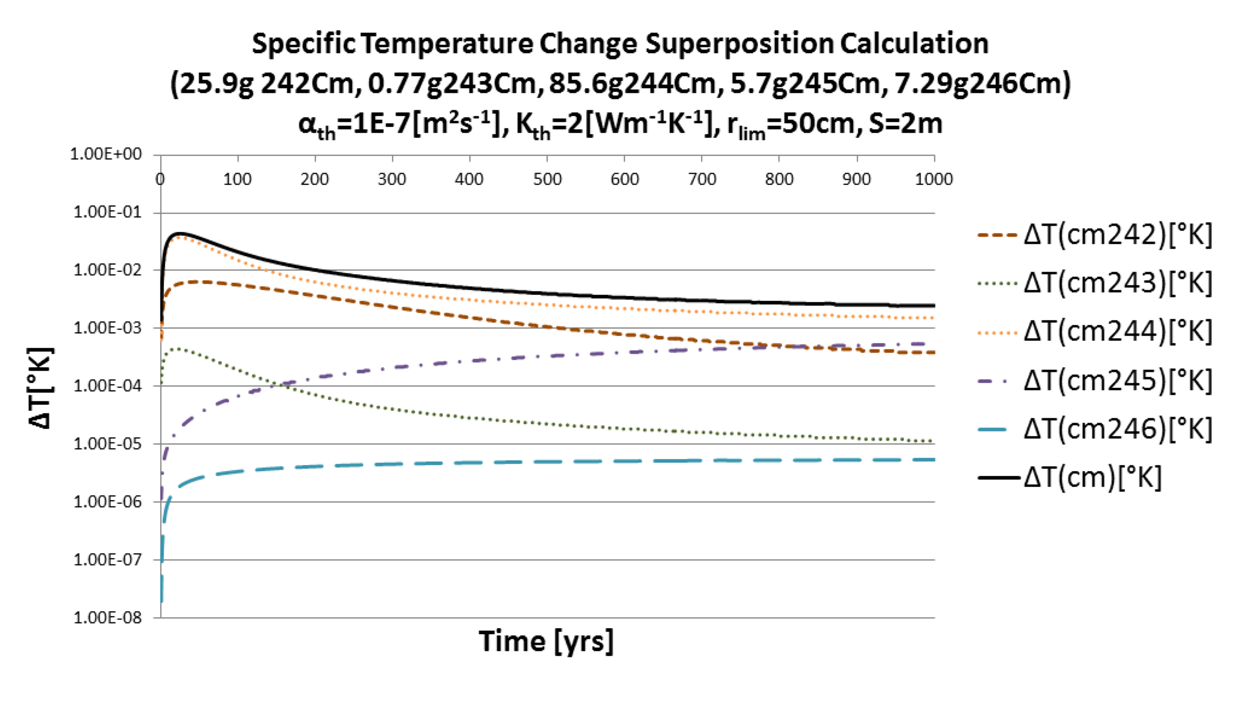
\includegraphics[width=\columnwidth]{images/CmSuperposition.eps}
\end{center}
\caption{As a demonstration of the calculation procedure, scaled temperature change 
  curves for two isotopes are superimposed to achieve a total temperature 
change (note log scale).}
\label{fig:CmSuperposition}
\end{figure}

%\begin{align}
%  T_{line}(t,x,y,z) &= \frac{1}{8\pi K_{th}} 
%  \bigintsss_0^t\!\frac{q_L(t')}{t-t'}e^{ \frac{-\left(x^2 + z^2\right)}{4\alpha 
%  (t-t')} }\nonumber\\ &\cdot\left[ \erf{\left[ \frac{1}{2} \frac{\left( y + 
%  \frac{L}{2} \right)}{\sqrt{\alpha(t-t')}}  \right]} - \erf{\left[ \frac{1}{2} 
%  \frac{\left( y - \frac{L}{2} \right)}{\sqrt{\alpha(t-t')}}  \right]} 
%  \right]\,\mathrm{dt'},
%  \label{line}
%  \intertext{adjacent packages within the central tunnel are represented by the 
%  point source solution }
%  T_{point}(t,r) &= 
%  \frac{1}{8K_{th}\sqrt{\alpha}\pi^{\frac{3}{2}}}\bigintsss_0^{-t}\!\frac{q(t')}{(t-t')^{\frac{3}{2}}}e^{\frac{-r^2}{4\alpha(t-t')}}\,\mathrm{dt'},
%  \label{point}
%  \intertext{and adjacent disposal tunnels are represented by infinite line 
%  source solutions}
%  T_{\infty line}(t,x,z) &= \frac{1}{4\pi K_{th}} 
%  \bigintsss_0^t\!\frac{q_L(t')}{t-t'}e^{ \frac{-\left(x^2 + z^2\right)}{4\alpha 
%  (t-t')} }
%  \intertext{in infinite homogeneous media, where}
%  \label{infline}
%  \alpha &= ~~\mbox{thermal diffusivity } [m^2\cdot s^{-1}]\nonumber\\
%  q(t) &= ~~\mbox{point heat source} [W]\nonumber\\
%  \intertext{and}
%  q_L(t) &= ~~\mbox{linear heat source} [W\cdot m^{-1}]\nonumber
%\end{align}
%Superimposed point and line source solutions allow for a notion of the 
%repository layout to be modeled in the host rock.


% How did you get such fabulous results?
%       in reproducible detail

% Specific Temperature Change

% Runs of the LLNL model (range table)

% Supporting data from Joe Carter (heat per iso)

% Interpolation (figure this out, or be vague?)

% Incorporation in Cyder (discuss capacity estimation, briefly.)

\section{Results and Analysis}
% Provide your results:
%       clearly

The primary outcome of this work is a mulitdimensional database of repository temperature 
change per mass of high heat contributing isotopes as a function of waste
package spacing and thermal parameters of the host geology, $\alpha_{th}$ and $K_{th}$. 
Results of unit tests and benchmarking efforts concerning this tool will be described in this 
section, as will a proof of principle base case demonstration of its use. 

% Unit Test Results

Unit tests are a way to check that your code works. Unit tests performed on 
these analytics tested the behavior of the interpolation and specific 
temperature change algorithms.

% Benchmarking Efforts

Comparing the results of this method with the \gls{LLNL} model gave 
appropriately similar results. 


% Base Case Demonstration ???
The base case demonstration of integration with the Cyclus next generation 
fuel cycle simulator.

\section{Conclusions}
% Was: Importance to Others - Replace with a conclusion.
The Cyder source code in which these models are implemented as well as 
associated documentation are freely available for use by model developers in the 
field of nuclear waste management. The application programming interface to this 
software library is intentionally general to facilitate the incorporation of the 
models presented here within software tools in need of a multicomponent repository 
model.

Furthermore, this work contributes to an expanding ecosystem of computational 
models available for use with the Cyclus fuel cycle simulator. This hydrologic 
nuclide transport library, by virtue of its capability to modularly integrate 
with the Cyclus fuel cycle simulator has laid the foundation for integrated 
disposal option analysis in the context of fuel cycle options. 

%%%%%%%%%%%%%%%%%%%%%%%%%%%%%%%%%%%%%%%%%%%%%%%%%%%%%%%%%%%%%%%%%%%%%%%%%%%%%%%%
%\nocite{*}
\bibliographystyle{ans}
\bibliography{bibliography}
\end{document}



